\documentclass[12pt]{article}
\usepackage{amsmath}
\usepackage{graphicx}

\title{Word Count MapReduce Implementation}
\author{Le Duy Anh}
\date{3/12/2024}

\begin{document}

\maketitle

\begin{abstract}
This report describes the implementation of a Word Count problem using a custom MapReduce-like approach in C++. The program utilizes multi-threading with `std::thread` and synchronization via `std::mutex` to efficiently count the frequency of words across multiple input text files.
\end{abstract}

\section{Introduction}
The Word Count problem is a classic example of distributed computing, where the goal is to count the frequency of each word in a large collection of text. In this implementation, we aim to process multiple text files in parallel using threads, similar to a MapReduce framework, to increase performance. The program employs a custom implementation of a Mapper and Reducer to count words concurrently.

\section{Choice of MapReduce Implementation}
The decision to implement this problem using threads and a shared hash map was driven by the need for efficiency and parallel processing. The program processes multiple input files concurrently by creating a thread for each file. Each thread reads the contents of the file, counts word occurrences locally, and then merges the results into a shared global word count map in a thread-safe manner using a mutex. This approach simulates a MapReduce-style system, where the map phase is executed in parallel, and the reduce phase merges the results from all threads.

The choice of this specific implementation is primarily based on the following factors:
\begin{itemize}
    \item \textbf{Concurrency}: The program uses multi-threading to process multiple files in parallel, improving performance for large datasets.
    \item \textbf{Thread Safety}: The use of `std::mutex` ensures that the shared data structure (the global word count map) is protected from race conditions.
    \item \textbf{Simplicity}: While this isn't a full-fledged MapReduce framework, the threading model is simple to implement and effective for this problem.
\end{itemize}

\section{Mapper and Reducer}
In this custom MapReduce implementation, the Mapper and Reducer roles are handled as follows:

\subsection{Mapper}
The Mapper function, `countWordsInFile`, reads each file word by word. For each word, the Mapper:
\begin{itemize}
    \item Converts the word to lowercase.
    \item Removes punctuation characters.
    \item Increments the count of the word in a local map for that specific thread.
\end{itemize}
This local map is stored in a `std::unordered\_map` for each thread.

\subsection{Reducer}
The Reducer function is responsible for merging the local maps from each thread into a global word count map. This process is synchronized using a `std::mutex` to prevent concurrent access to the global map. The final word count map contains the total word frequencies for all input files.

\section{Flowchart of the Process}
The following figure illustrates the flow of data through the Mapper and Reducer steps:

\begin{figure}[h!]
\centering
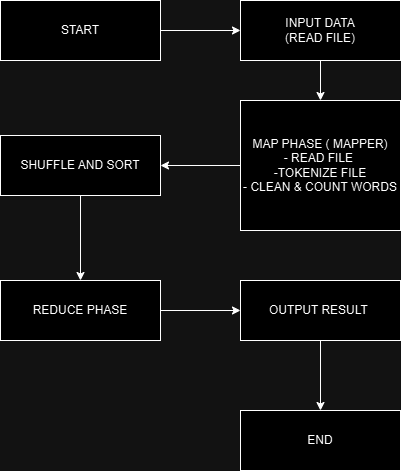
\includegraphics[width=0.8\textwidth]{mapreduce_flowchart.png}
\caption{Flowchart of the Mapper and Reducer process}
\label{fig:flowchart}
\end{figure}

\section{Conclusion}
The custom MapReduce-like implementation of the Word Count problem demonstrates the effectiveness of multi-threading for parallel processing. The use of a mutex ensures that the shared data is updated safely, and the final word count is computed efficiently by leveraging concurrency. This approach can be expanded into a more complete MapReduce framework, but it is a useful and scalable method for relatively smaller datasets.

\end{document}
